\documentclass{beamer}

\usepackage{amsmath,amssymb,amsfonts}
\usepackage{array}
\usepackage[british]{babel}
\usepackage{bbm}
\usepackage{bbold}
\usepackage{beamerthemesplit}
\usepackage[bf]{caption}
\usepackage{cite}
\usepackage{color}
\usepackage{enumerate}
\usepackage{eurosym}
\usepackage{graphicx}
\usepackage{rotating}
\usepackage{slashed}
\usepackage[utf8]{luainputenc}
\usepackage{xcolor}
\usepackage{array}
\usepackage{listings}
\usepackage{nicefrac} % for \nicefrac macro giving nice fractions in exponent
\usepackage{enumerate}

\usepackage{pgfplots}
\pgfplotsset{compat=1.10}

% My fonts:
% ---------
\usepackage{libertine}
\usefonttheme[onlymath]{serif}
\usepackage[activate]{microtype}

% My definitions:
% ---------------
\newcommand\NS{ N_{\scriptscriptstyle{\mathrm{S}}} }
\newcommand\GNewton{ G_{\scriptscriptstyle{\mathrm{N}}}{} }
\newcommand\SEH{ S_{\scriptscriptstyle{\mathrm{EH}}}{} }
\newcommand\SUV{ S_{\scriptscriptstyle{\mathrm{UV}}}{} }
\newcommand\Sbare{ S_{\scriptscriptstyle{\mathrm{bare}}}{} }
\newcommand\Sclass{ S_{\scriptscriptstyle{\mathrm{classical}}}{} }
\newcommand\MPl{ M_{\scriptscriptstyle{\mathrm{Pl}}}{} }
\newcommand\metric{ g_{\mu\nu} }

%----------------------------------------------------------------------------------------
% OTHER STUFF
%----------------------------------------------------------------------------------------

\newsavebox\bracebox

\makeatletter
\def\amsbb{\use@mathgroup \M@U \symAMSb}
\makeatother

\usetheme{Boadilla}

\setbeamertemplate{section in toc}[sections numbered]
\setbeamertemplate{blocks}[rounded][shadow=false]
\setbeamertemplate{itemize items}[default]
\beamertemplatenavigationsymbolsempty
\setbeamercolor{footline}{bg=black}
\setbeamertemplate{footline}{%
  \raisebox{8pt}{\makebox[\paperwidth]{\hfill\makebox[15pt]{{\tiny\insertframenumber}}\qquad}}
}

\definecolor{myred}{RGB}{176,50,50}
\definecolor{myblue}{RGB}{50,50,176}
\definecolor{mygreen}{RGB}{60,166,60}

\newcommand\blfootnote[1]{%
  \begingroup
    \renewcommand\thefootnote{}\footnote{#1}%
    \addtocounter{footnote}{-1}%
    \endgroup
}

%----------------------------------------------------------------------------------------
% DOCUMENT
%----------------------------------------------------------------------------------------

\begin{document}

%%%%%%%%%%%%%%%%%%%%%%%%%%%%%%%%%%%%%%%%%%
%%%   TITLE SLIDE
%%%%%%%%%%%%%%%%%%%%%%%%%%%%%%%%%%%%%%%%%%

\title{Matter fields in the Asymptotic Safety scenario}
\author{Peter Labus}
\institute{SISSA Trieste
  \vspace{5mm}
  \\ \vspace{8pt}PL, T. R. Morris and Z. H. Slade, Phys. Rev. D 94 (2016)
  \\ \vspace{8pt}P. Don\`a, A. Eichhorn, PL and R. Percacci, Phys. Rev. D93 (2016)
  \\ \vspace{8pt}PL, R. Percacci, G.P. Vacca, Phys. Lett.  B753 (2016)
  \\ \vspace{8pt}A. Eichhorn, PL, J. M. Pawlowski, M. Reichert, \textit{In preparation.}
  \date{14/09/2017}
}
\begin{frame}[noframenumbering,plain]
  \titlepage
\end{frame}

%----------------------------------------------------------------------------------------
%   Section 1 --- Quantum Gravity
%----------------------------------------------------------------------------------------

\section{Asymptotically safe quantum gravity}
\fontsize{10pt}{7.2}\selectfont

%%%%%%%%%%%%%%%%%%%%%%%%%%%%%%%%%%%%%%%%%%
%%%   SLIDE 0
%%%%%%%%%%%%%%%%%%%%%%%%%%%%%%%%%%%%%%%%%%

% TODO:

\begin{frame}
  \frametitle{Outline}
  \begin{enumerate}[I]
    \item
      Asymptotic Safety
      \begin{itemize}
        \item Why quantum gravity?
        \item What is asymptotic safety and why to study it?
      \end{itemize}
      \vfill
    \item
      Matter fields coupled to gravity
      \begin{itemize}
        \item Why we should include matter fields from the start...
        \item ...and what we might learn from it
      \end{itemize}
      \vfill
    \item
      Tools to study asymptotic safety
      \begin{itemize}
        \item What is needed and available?
        \item Why to use the functional renormalisation group (FRG)?
      \end{itemize}
      \vfill
    \item
      Known issues of the FRG in gravity
      \begin{itemize}
        \item Outline of some open research questions...
        \item ...and relation to my own work
      \end{itemize}
      \vfill
    \item
      My research \& its implications
  \end{enumerate}
\end{frame}

%%%%%%%%%%%%%%%%%%%%%%%%%%%%%%%%%%%%%%%%%%
%%%   SLIDE 1
%%%%%%%%%%%%%%%%%%%%%%%%%%%%%%%%%%%%%%%%%%

% TODO:
% consistent spacing
% maybe only one question on last version of slide

\begin{frame}
  \frametitle{Why quantum gravity?}
  \textbf{Two pressing issues:}
  \begin{enumerate}
    \item singularities in GR (black holes, big bang)
      \hspace{2cm}
      \raisebox{-.5\height}{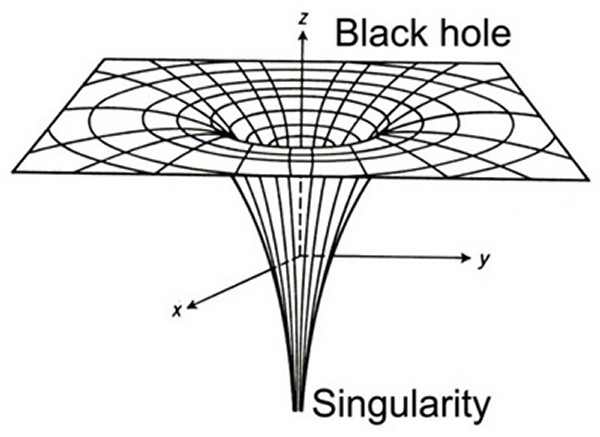
\includegraphics[width=0.25\textwidth]{blackholes_singularity.jpg}}
    \item singularities in SM (stability of $U(1)$ and Higgs sector)
      % \hspace{1cm}
      \raisebox{-.5\height}{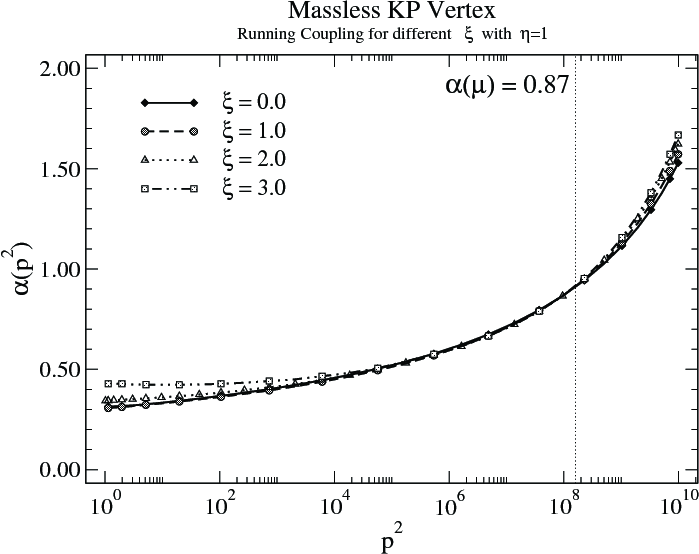
\includegraphics[width=0.25\textwidth]{running_alpha.png}}
  \end{enumerate}
  \vfill
  \pause
  \textbf{More theoretical issues:}\\[5pt]
  cosmological constant problem, hierarchy problem, origin of symmetries and field content,
  CP-violation, grand unification?, TOE?, \dots
\end{frame}

\addtocounter{framenumber}{-1}
\begin{frame}
  \frametitle{Why quantum gravity?}
  \textbf{Two pressing issues:}
  \begin{enumerate}
    \item singularities in GR (black holes, big bang)
      \hspace{2cm}
      \raisebox{-.5\height}{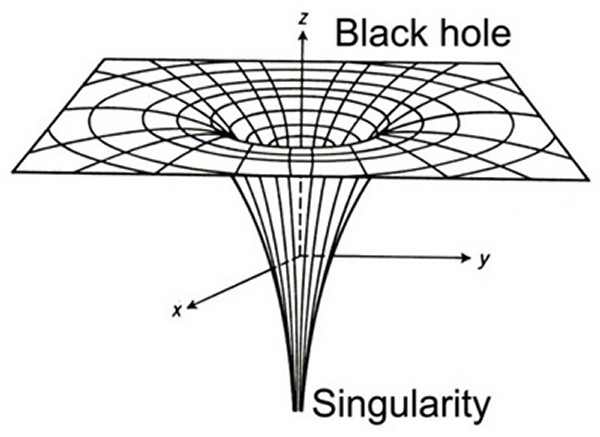
\includegraphics[width=0.25\textwidth]{blackholes_singularity.jpg}}
    \item singularities in SM (stability of $U(1)$ and Higgs sector)
      % \hspace{1cm}
      \raisebox{-.5\height}{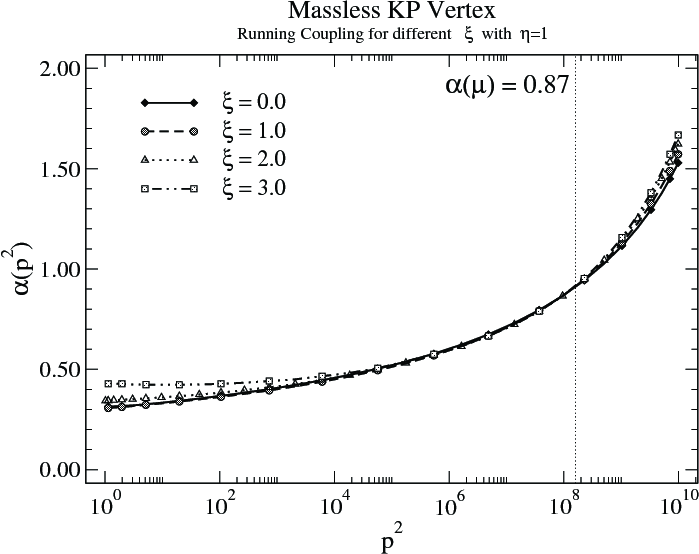
\includegraphics[width=0.25\textwidth]{running_alpha.png}}
  \end{enumerate}
  \vfill
  \begin{center}
    \fontsize{12pt}{7.2}\selectfont
    \textbf{ Can one help to cure the other? }
    \raisebox{-.5\height}{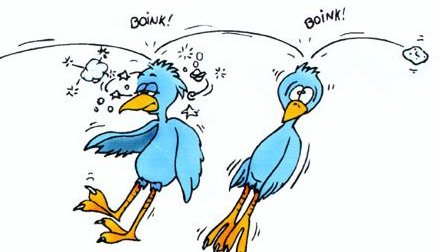
\includegraphics[width=0.25\textwidth]{two_birds.jpg}}
  \end{center}
  \pause
  \begin{center}
    candidates:\\[5pt]
    string theory, loop quantum gravity, causal dynamical triangulation, Regge calculus,\\
    causal sets, spin foams, group field theory, \dots
  \end{center}
\end{frame}

\addtocounter{framenumber}{-1}
\begin{frame}
  \frametitle{Why quantum gravity?}
  \textbf{Two pressing issues:}
  \begin{enumerate}
    \item singularities in GR (black holes, big bang)
      \hspace{2cm}
      \raisebox{-.5\height}{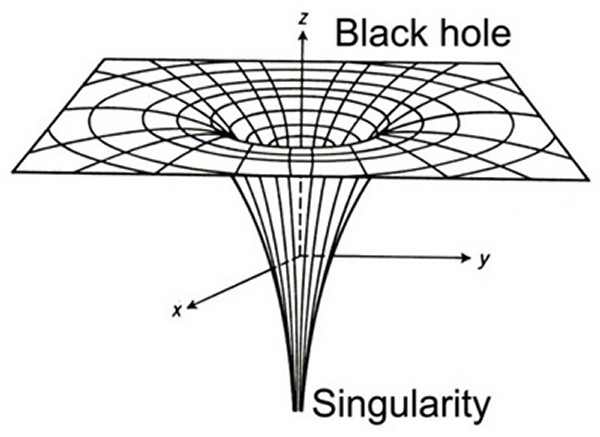
\includegraphics[width=0.25\textwidth]{blackholes_singularity.jpg}}
    \item singularities in SM (stability of $U(1)$ and Higgs sector)
      % \hspace{1cm}
      \raisebox{-.5\height}{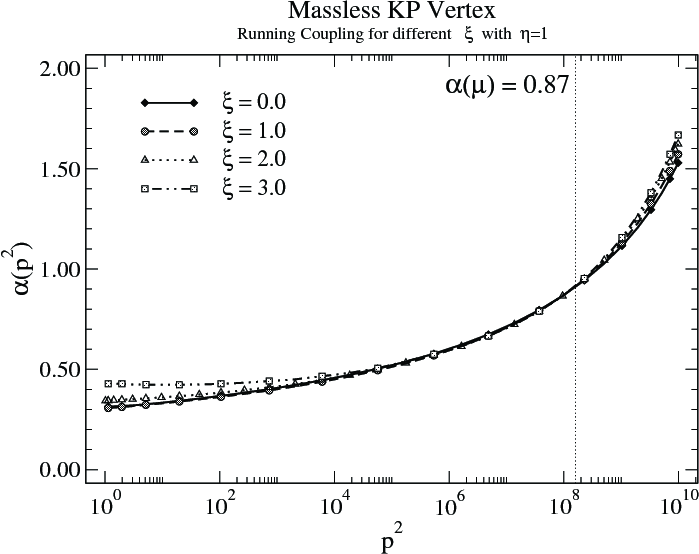
\includegraphics[width=0.25\textwidth]{running_alpha.png}}
  \end{enumerate}
  \vfill
  \begin{center}
    \fontsize{12pt}{7.2}\selectfont
    \textbf{ Can one help to cure the other? } \\[15pt]
    \textbf{ Have to go beyond QFTs? }
  \end{center}
\end{frame}

%%%%%%%%%%%%%%%%%%%%%%%%%%%%%%%%%%%%%%%%%%
%%%   SLIDE 2
%%%%%%%%%%%%%%%%%%%%%%%%%%%%%%%%%%%%%%%%%%

% TODO:
% references
% check formula
% Feynman diagram of graviton scattering
% picture of Einstein?

\begin{frame}
  \frametitle{But wait a minute...!}
  \textbf{We know (low-energy) quantum gravity:}\\[5pt]
  GR as an EFT $\rightarrow$ can calculate corrections to Newtonian potential [Donogue et al.]
  \begin{align*}
    \boxed{
      V(r) = -\frac{\GNewton m_1 m_2}{r}
      \bigg(
        1
        + 3 \, \frac{\GNewton (m_1 + m_2)}{r \, c^2}
        + \frac{41}{10 \pi} \, \frac{\GNewton \hbar}{r^2 \, c^3}
        + \dots
      \bigg)
    }
  \end{align*}
  \hfill Probably most accurate result in quantum gravity...!
  \pause
  \vfill
  \begin{itemize}
    \item well-defined QFT of gravity\\[5pt]
    \item predictive, but experimentally indistinguishable from GR\\[5pt]
    \item consistent with all available data
  \end{itemize}
\end{frame}

\addtocounter{framenumber}{-1}
\begin{frame}
  \frametitle{But wait a minute...!}
  \textbf{We know (low-energy) quantum gravity:}\\[5pt]
  GR as an EFT $\rightarrow$ can calculate corrections to Newtonian potential [Donogue et al.]
  \begin{align*}
    \boxed{
      V(r) = -\frac{\GNewton m_1 m_2}{r}
      \bigg(
        1
        + 3 \, \frac{\GNewton (m_1 + m_2)}{r \, c^2}
        + \frac{41}{10 \pi} \, \frac{\GNewton \hbar}{r^2 \, c^3}
        + \dots
      \bigg)
    }
  \end{align*}
  \hfill Probably most accurate result in quantum gravity...!
  \pause
  \vfill
  \begin{center}
    \fontsize{12pt}{7.2}\selectfont
    \textbf{ So, what's the catch? }
  \end{center}
  \pause
  \vspace{10pt}
  Expansion in $\nicefrac{k}{\MPl}$ needs $\infty$--terms in UV:\\[5pt]
  \begin{itemize}
    \item How to make predictions at the Planck scale?\\[5pt]
    \item Can we address either of our two issues?
  \end{itemize}
\end{frame}

%%%%%%%%%%%%%%%%%%%%%%%%%%%%%%%%%%%%%%%%%%
%%%   SLIDE 3
%%%%%%%%%%%%%%%%%%%%%%%%%%%%%%%%%%%%%%%%%%

% TODO:
% picture Feynman?

\begin{frame}
  \frametitle{The path integral approach}
  % \textbf{Have to make sense of}
  \begin{align*}
    \boxed{
    \int \mathcal D \Phi \; e^{i S[\Phi]}\,,
    \text{ let's try } \Phi = \metric \,.
    }
  \end{align*}
  \vfill
  % Have to specify:
  \begin{itemize}
    \item integration measure $\mathcal D \metric$ (integral over all space-times)
    \item action $S[\metric]$
  \end{itemize}
  \vfill
  \begin{enumerate}
    \item $S[\metric] = \SEH[\metric] = - \frac{1}{16 \pi \GNewton} \int \sqrt{g} \, R$
      \hspace{2pt}
      \textit{does not work} [t'Hooft, Veltman]\\[15pt]
    \item $S = \Sbare = \SUV = \, ???\,,$\\[5pt]
          $S \neq \Sclass$
  \end{enumerate}
\end{frame}

\addtocounter{framenumber}{-1}
\begin{frame}
  \frametitle{The path integral approach}
  % \textbf{Have to make sense of}
  \begin{align*}
    \boxed{
    \int \mathcal D \Phi \; e^{i S[\Phi]}\,,
    \text{ let's try } \Phi = \metric \,.
    }
  \end{align*}
  \vfill
  % Have to specify:
  \begin{itemize}
    \item integration measure $\mathcal D \metric$ (integral over all space-times)
    \item action $S[\metric]$
  \end{itemize}
  \vfill
  \begin{center}
    \fontsize{12pt}{7.2}\selectfont
    \textbf{ What is going wrong here? }
  \end{center}
  \begin{columns}[T]
    \begin{column}{.5\textwidth}
      \begin{center}
        couplings of the theory are \textbf{scale-dependent},\\[10pt]
        na\"ively $\GNewton \rightarrow \infty$ in the UV limit
      \end{center}
    \end{column}
    \begin{column}{.5\textwidth}
      \begin{center}
        vacuum polarisation in QED:
        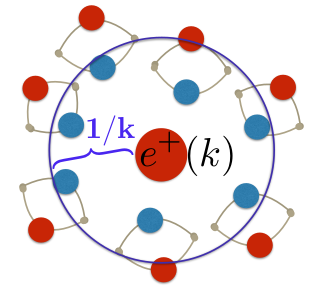
\includegraphics[width=0.4\textwidth]{screening.png}
      \end{center}
    \end{column}
  \end{columns}
\end{frame}

%%%%%%%%%%%%%%%%%%%%%%%%%%%%%%%%%%%%%%%%%%
%%%   SLIDE 4
%%%%%%%%%%%%%%%%%%%%%%%%%%%%%%%%%%%%%%%%%%

% TODO:

\begin{frame}
  \frametitle{A look into theory space}
  \textbf{effective average action}
  \begin{align*}
    \boxed{
    e^{ - \Gamma_k \lbrack \varphi \rbrack }
    = \int \mathcal D \chi \;
    e^{
      - S \lbrack \chi + \varphi \rbrack
      - \Delta S_k \lbrack \chi \rbrack
      + \int \mathrm d^dx \;
      \frac{ \delta \Gamma_k }{ \delta \varphi (x) }
      \, \chi(x)
    }
    }
  \end{align*}
  \vspace{2pt}

  \begin{columns}[T]
    \begin{column}{.4\textwidth}
      \textbf{Theory space:}\\[5pt]
      QFT = trajectory in theory space,
      parametetrised by scale $k$\\[25pt]
      % \begin{center}
        \includegraphics[scale=0.6]{theory_space.pdf}
      % \end{center}
    \end{column}
    \begin{column}{.6\textwidth}
      \begin{center}
        $\Gamma_k \lbrack \varphi \rbrack = \sum_n \, g_n(k) \; \mathcal O_n(\varphi, \partial)$\\[5pt]
        all operators allowed by symmetry\\[3pt]
        (generated by quantum fluctuations)\\[20pt]
        \pause
        \textbf{Q:} All $g_n(k)<\infty$ for all $k$?\\[5pt]
        \textbf{A:} Ultra violet \textbf{fixed point}!
      \end{center}
    \end{column}
  \end{columns}
\end{frame}

\addtocounter{framenumber}{-1}
\begin{frame}
  \frametitle{A look into theory space}
  \vspace{7.5pt}
  \textbf{effective average action}
  \begin{align*}
    \boxed{
    e^{ - \Gamma_k \lbrack \varphi \rbrack }
    = \int \mathcal D \chi \;
    e^{
      - S \lbrack \chi + \varphi \rbrack
      - \Delta S_k \lbrack \chi \rbrack
      + \int \mathrm d^dx \;
      \frac{ \delta \Gamma_k }{ \delta \varphi (x) }
      \, \chi(x)
    }
    }
  \end{align*}
  \vspace{2pt}

  \begin{columns}[T]
    \begin{column}{.6\textwidth}
        UV critical surface:\\[10pt]
      % \begin{center}
        \includegraphics[scale=0.6]{uvcritsurface_talk.pdf}
      % \end{center}
    \end{column}
    \begin{column}{.4\textwidth}
      \begin{center}
        fixed point in $\infty$--dim theory space:\\
        \textbf{asymptotic safety} (freedom)\\[20pt]
        relevant directions\\[3pt]
        $\rightarrow$ free parameters (fix in the IR)\\[10pt]
        irrelevant directions\\[3pt]
        $\rightarrow$ predictions of the theory
      \end{center}
    \end{column}
  \end{columns}
\end{frame}

%%%%%%%%%%%%%%%%%%%%%%%%%%%%%%%%%%%%%%%%%%
%%%   SLIDE 5
%%%%%%%%%%%%%%%%%%%%%%%%%%%%%%%%%%%%%%%%%%

% TODO:

\begin{frame}
  \frametitle{Asymptotically safe (pure) gravity }
\end{frame}

\section{Matter fields in asymptotic safety}

\section{Technical tools}

\section{Known issues}

\begin{frame}
  \frametitle{Truncating the exact renormalisation group equation}

  \begin{columns}[T]

    \begin{column}{.5\textwidth}
      \begin{center}
        \textbf{derivative expansion:}
        \begin{itemize}
          \item
            expanded in diffeomorphism invariant quantities
            ($R$, $R_{\mu\nu}$, $C_{\mu\nu}$, ...)
          \item
            background field approximation + heat kernel
            techniques
          \item
            using curved backgrounds
            $\rightarrow$ physically most relevant?
          \item
            functional truncations
            $\rightarrow$ $\infty$-many operators
          \item
            $\beta_{\GNewton}$ receives contributions
            from cutoff--operator
        \end{itemize}
      \end{center}
    \end{column}

    \begin{column}{.5\textwidth}
      \begin{center}
        \textbf{vertex expansion:}
        \begin{itemize}
          \item
            local, non-diffeomorphism invariant action $\Gamma_k$
            $\rightarrow$ but maybe \textit{effective universality}?
          \item
            calculate Feynman diagrams
          \item
            many different ``avatars'' of $\GNewton$
          \item
            (usually) evaluated on flat background
            $\rightarrow$ farther from ``true vacuum''?
          \item
            functional truncations difficult
          \item
            fluctuation field couplings do not receives contributions
            from cutoff--operator
        \end{itemize}
      \end{center}
    \end{column}

  \end{columns}
\end{frame}

\begin{frame}
  \frametitle{Background (in-)dependence of the ERGE in gravity}
\end{frame}

%%%%%%%%%%%%%%%%%%%%%%%%%%%%%%%%%%%%%%%%%%
%%%   SLIDE
%%%%%%%%%%%%%%%%%%%%%%%%%%%%%%%%%%%%%%%%%%

% TODO:
\section{My research \& and its implications}

%%%%%%%%%%%%%%%%%%%%%%%%%%%%%%%%%%%%%%%%%%
%%%   SLIDE
%%%%%%%%%%%%%%%%%%%%%%%%%%%%%%%%%%%%%%%%%%

% TODO:

\fontsize{8pt}{7.2}\selectfont
\begin{frame}
  \frametitle{Overview of my research}
  \vspace{3pt}

  \begin{columns}[T]
    \begin{column}{.8\textwidth}
      \begin{enumerate}[a]

        \sbox\bracebox{%
          \begin{minipage}{.8\linewidth}%
          \item
            \textbf{functional truncations} of non-minimally coupled
            scalar fields\\[3pt]
            [Percacci, Vacca '15; PL, Percacci, Vacca '16]
            \begin{itemize}
              \fontsize{8pt}{7.2}\selectfont
              \item Are there scaling solutions?
              \item What is the impact of the scalars?
            \end{itemize}
            \vspace{5pt}

          \item renormalisation group dynamics of \textbf{gravity-matter vertices}\\[3pt]
            [Don\`a, Eichhorn, PL, Percacci '16]
            \begin{itemize}
              \fontsize{8pt}{7.2}\selectfont
              \item Are there well-behaved fixed points?
              \item How does this compare to other truncations?
            \end{itemize}
            \vspace{5pt}

          \item
            \textbf{effective universality}\\
            and subtracting the cutoff--dependence using the msWI\\[3pt]
            [Eichhorn, PL, Pawlowski, Reichert '17]
          \end{minipage}%
        }\usebox{\bracebox}%
        \makebox[15pt][r]{$\left.\vrule height\ht\bracebox width 0pt\right\}$}

            \vspace{15pt}
        \sbox\bracebox{%
          \begin{minipage}{.8\linewidth}%
          \item
            \textbf{ERGE \& msWI}\\[3pt]
            [Dietz, Morris '15; PL, Morris, Slade '16; Percacci, Vacca '16]
            \begin{itemize}
              \fontsize{8pt}{7.2}\selectfont
              \item Can they be solved together?
              \item Are there restrictions to RG properties (FPs, number of relevant directions, etc.)?
            \end{itemize}
          \end{minipage}%
        }\usebox{\bracebox}%
        \makebox[15pt][r]{$\left.\vrule height\ht\bracebox width 0pt\right\}$}

    \end{enumerate}
  \end{column}

  \hspace{-2.5cm}
  \begin{column}{.2\textwidth}
    \begin{center}
      \vspace{53pt}
      gravity\\[2pt]
      $\oplus$\\[3pt]
      $\NS$ scalar fields\\
      \vspace{108pt}
      CORE gravity
    \end{center}
  \end{column}
\end{columns}
\end{frame}

\begin{frame}
  \titlepage
\end{frame}

\end{document}
